\documentclass[a4paper]{article}

%% Language and font encodings
\usepackage[english]{babel}
\usepackage[utf8x]{inputenc}
\usepackage[T1]{fontenc}

%% Sets page size and margins
\usepackage[a4paper,top=3cm,bottom=2cm,left=3cm,right=3cm,marginparwidth=1.75cm]{geometry}

%% Useful packages
\usepackage{amsmath}
\usepackage{graphicx}
\usepackage[colorinlistoftodos]{todonotes}
\usepackage[colorlinks=true, allcolors=blue]{hyperref}
\usepackage{indentfirst}

\title{Activity 1}
\author{Isaac Neri Gómez Sarmiento}
\date {January 27, 2018}

\begin{document}
\maketitle



\section{Introduction}

The goal of this activity is to familiarize with the \LaTeX\ syntaxis by doing a summary of the information found in Wikipedia about {\bf Atmosphere of Earth}. \par 


Earth's atmosphere is, in few words, the layer of gases that surrounds  Earth which is retained by Earth's gravity. It provides numerous benefits such as absorbing UV solar radiation, warming by heat retention, etc. 

\section{Atmosphere's composition}

As we can see from the chart below, the three main gases the Earth's atmosphere is made of are: Nitrogen, Oxygen and Argon. The other gases are called trace gases and some of them are the greenhouse gases. There are also other substances such as volcanic ashes or pollen, as well as industrial pollutants like aerosols which contain chlorine or fluorine.

\begin{figure}[h!]
\centering
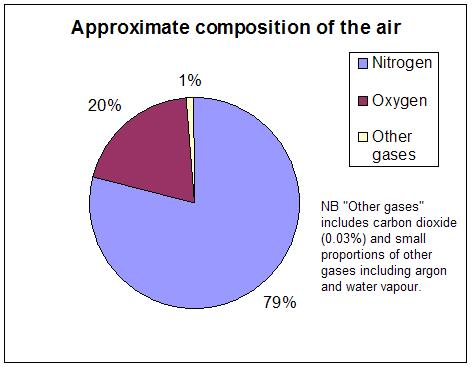
\includegraphics[width=0.5\textwidth]{Air_composition_pie_chart}
\caption{\label{fig:Atmosphere Pie Chart}Atmospheric gases distribution}
\end{figure}


\section{Structure of the atmosphere}
Atmosphere of Earth is composed of 5 main layers: Troposphere, Stratosphere, Mesosphere, Thermosphere and Exosphere. Generally, the air pressure and density increases as altitude does. It's temperature that doesn't follow that behavior, some layers are colder or hotter than the others, it may stay constant or increase depending on the altitude. 


\begin{table}[h!]
\centering
\begin{tabular}{l|r}
\centering
Atmospheric Layer & Altitude \\\hline
Exosphere & 700-10,000 km \\
Thermosphere & 80-700 km\\
Mesosphere & 50-80 km \\
Stratosphere & 12-50 km \\
Troposphere & 0-12 km
\end{tabular}
\caption{\label{tab:widgets}Atmospheric layer altitudes}
\end{table}

\subsection{Exosphere}
It is the outermost layer of the Earth’s Atmosphere which is mainly composed of extremely low density hydrogen, helium and some other heavier molecules such as nitrogen or oxygen. One particularity it’s that molecules found in this layer are too far apart and no longer behave like gases so they tend to escape into space. 

\subsection{Thermosphere}
It is the second-highest layer of Earth's atmosphere. Its height may vary depending on changes in solar activity. Its temperature gradually increases with altitude that it can even reach 1500$^{\circ}$. This layer is cloudless and free of water vapor, nonetheless, this is where aurora borealis and australis take place.

\subsection{Mesosphere}
It is the third highest layer of Earth's atmosphere.As altitude increases in this layer, the temperature drops.It is the coldest place on Earth with an average of -85$^{\circ}$. The temperature is so cold that the water vapor sublimates and turns into  tiny ice crystals. These crystals create noctilucent clouds. In this layer most of the meteors burn up when they enter. 

\subsection{Stratosphere}
It is the second-lowest layer of Earth's atmosphere. The atmospheric pressure is to low, compared to the sea level is approximately 1/1000. The ozone layer it's located in this layer. Temperature increases as altitude does due to the absorption of UV radiation by the ozone layer. 

\subsection{Troposphere}
It's the lowest layer which comprises Earth's surface and goes up to 12 km approximately. Unlike the stratosphere or the thermosphere, as altitude increases the temperature drops, due to the transfer of energy from the surface. The earth's surface is then the warmest section of this layer. It contains almost 80\% of the mass of the earth atmosphere, that means that it's the most dense atmospheric layer of all. 

\section{Physical Properties}
Earth's atmosphere mass is about 5.15 x $10^{18}$ kg. The average sea level pressure and density is about 101,325 pascals and $1.2 kg/m^3$ respectively. Density decreases at an exponential rate by a factor of 1/e every 7.64 km. As for temperature, it decreases with altitude from the sea level, but as soon as we reach the troposphere, temperature starts to increase. It's in that layer that atmospheric circulation takes place, that is, the movement of air and heat distribution around the Earth. Temperature is a variable that it's taken into consideration when measuring the speed of sound. 

\section{Optical Properties}

\begin{enumerate}
{\bf \item  Scattering}
\\
This property is present in earth when light reaches the earth and deviate from  its straight trajectory. If light doesn't interact with atmosphere, then it's called direct radiation. In the other hand, if light does interact with it, it's called indirect radiation. Examples of scattering are the light that goes through clouds or the  scattering of blue wavelengths by the molecules of the atmosphere that are bigger than the blue wavelength (which is the reason the sky is blue). 
{\bf \item Absorption }
\\
Molecules absorb different light wavelengths, increasing their energy and heating the atmosphere. 
{\bf \item Emission}
\\
After a body absorbs energy, it might emit it with a certain wavelenght depending on its temperature. Hotter objects emit more radiation with shorter wavelengths and colder objects emit less radiation with longer wavelengths. Atmosphere emits infrared radiation due to its temperature. 
{\bf \item Refractive Index}
\\
The refractive index it's a measure of how lights propagates through a medium.It determines by how much the speed of light is reduced. In air, the speed of light it's not that much affected, since its refractive index is about  1.000277, meaning that light goes 1.000277 slower. 
\end{enumerate}

\section{Appendix}
{\parindent0pt
{\bf 1. What got your attention in this activity?}

The many web resources that you can access to write in \LaTeX. The activity refreshed my knowledge about the structure of the atmosphere.

{\bf2. What did you find the least interesting?}

Nothing. Everything was interesting. 

{\bf 3. What changes would you make in order to improve this activity?}

That we can choose another topic.


{\bf4. What was you first impression using \LaTeX\ ? }

At first it seemed kind of difficult. I first tried to use CoCalc to do the activity, but I found Overleaf to be more user-friendly. As we work on the activities, we'll be able to learn more commands. 

{\bf 5. Was it enough the time provided? }

Yes, for this activity 2 or 3 days would be enough to finish it. One week might be necessary as soon as we start coding with Python. 

{\bf 6. Did you find a document or an online resource you might share with the others?}

Yes, that they should try Overleaf.


\section{References}

\begin{itemize}
  \item Atmosphere of Earth.  Retrieved January 27, 2018, from \url{https://en.wikipedia.org/wiki/Atmosphere_of_Earth}
  \item List of refractive indices.  Retrieved January 27, 2018, from \url{https://en.wikipedia.org/wiki/List_of_refractive_indices}
  \item {\bf Figure 1} retrieved January 27, 2018, from
\url{https://upload.wikimedia.org/wikipedia/commons/6/66/Air_composition_pie_chart.JPG}
\end{itemize} 



\end{document}